\section{3. Phylogenetics and tree reconstruction}

\begin{framed}
\textbf{Learning outcomes}\\
\begin{itemize}
\item 1
\item 2
\item 3
\end{itemize}
\end{framed}

In this chapter you will learn to use a \textit{Multiple Sequence Alignment} (MSA), like the ones you compiled in \href{/chapter2}{chapter 2}, and visualize the variation it contains as a phylogenetic tree.
A phylogenetic tree is considered a highly efficient \textit{data structure} summarizing the data and its variation contained in your MSA.
A tree is built from \textit{characters} which are the individual columns or positions in your MSA.
Characters have states, which are in this case the individual nucleotide or amino acid \textit{substitutions} occurring in that position (see Characters~&~trees below).
Invariable characters are columns or positions `occupied' by just one type of nucleotide or amino acid, whereas variable characters may have up to 4 different nucleotides or up to 20 amino acids per position.

% #%Create cross-link to MSA in chapter 2 when written

DNA and amino acid (AA) sequences contain the information necessary for building protein structure, comparing them in an MSA will enable insight how these structures, and their associated functions, may have changed over evolutionary times since they descended from an ancestral sequence.
The more character state changes (i.e., substitutions) occur between sequences, the more \textit{diverged} they are and probably also less related (see Related,~diverged below), and hence the further apart they will occur on your phylogenetic tree.
The information contained in your tree is hierarchical in nature, meaning that it is built-up as nested sets of subtrees that are also known as \textit{clades}.
A \textit{clade} is a group containing an ancestor together with all its descendants and is also referred to as a \textit{monophyletic} group.


\bigskip
\centerline{\rule{13cm}{0.4pt}}
\bigskip

\subsubsection{Rationale}

% :::{figure} images/chapter3/tree-of-life.png
% :alt: The Tree of Life
% :width: 40%
% :name: tree_of_life
% align: center
% The Tree of Life. Dated in millions of years; \
% rooted with Eubacteria. Credits: {cite}`tree_of_life_2022`.
% :::
% #% Unable to use figure tree_of_life due to copyright.

\begin{figure}[!htbp]
\centering
\includegraphics[width=0.5\linewidth]{files/tree-of-life_alt-af7529eddf9e121b8f98d25d1b99b119.png}
\caption[]{Simplified Tree of Life. Credits: \newline
\href{https://creativecommons.org/licenses/by/4.0/}{CC BY 4.0} \cite{tree_of_life_alt_2014}.}
\label{tree_of_life_alt}
\end{figure}

Why should we study phylogenetics and what is it about?
Ever since Darwin we know that all living things are connected in a tapestry of life, forming a phylogenetic tree of everything (Figure~\ref{tree_of_life_alt}).
Phylogenetics aims at understanding evolutionary relationships among genes, species, and higher taxa and as such it is relevant to almost all biological questions.
Why? Because an evolutionary context (rather than a `snapshot' perspective) allows identifying evolutionary lineages and their origins, and can provide information on how lifeforms and sequences change and adapt across millions of years.
Examples are studying the evolution of gene families within genomes, or the build-up of species relationships in a lineage.

\begin{figure}[!htbp]
\centering
\includegraphics[width=1\linewidth]{files/sars-cov-2-c625ea5bfa5a5808c0ab8b5230606e98.svg}
\caption[]{The SARS-CoV-2 phylogenetic tree, March 2024.
Credits: \href{https://creativecommons.org/licenses/by/4.0/}{CC BY 4.0} \cite{sars-cov-2_2018}.}
\label{sars-cov-2}
\end{figure}

Other examples are studying Covid-19 and other pathogen outbreaks (Figure~\ref{sars-cov-2}), studying molecular evolution and the accumulation of substitutions in a multiple sequence alignment (MSA).
Or, studying population history within a species, reconstructing historical biogeography: In all these cases having an \textit{accurate phylogenetic tree} is crucial, because we want to be able to reconstruct evolutionary lineages (the branches in phylogenetic trees) and how they evolved, changed, duplicated, or went extinct.
By \textit{accurate} we mean estimating relationships that are as close as possible to the actual (historic) relationships, which we cannot know for sure.
As they happened in the past we cannot \textit{prove} them, but they are hypotheses (of relationships) that we can only \textit{corroborate} (confirm, seek support for).

% :::{figure} images/chapter3/ancestral-states.png
% :alt: A phylogenetic tree with ancestral states
% :width: 100%
% :name: ancestral_states
% 
% Comparing species (or genes) in a phylogenetic tree allows inference of ancestral states and evolutionary trends.
% :::
% #% Unable to use figure ancestral_states because of poor quality

\begin{figure}[!htbp]
\centering
\includegraphics[width=1\linewidth]{files/ancestral-states_alt-7d2c296e2211f343a7dbc95928147ca9.pdf}
\caption[]{Comparing species (or genes) in a phylogenetic tree allows inference of ancestral states and evolutionary trends.
Credits: \href{https://creativecommons.org/licenses/by-nc/4.0/}{CC BY-NC 4.0} \cite{own_3_2024}.}
\label{ancestral_states_alt}
\end{figure}

When a phylogenetic tree is known for a specific group, and it is properly rooted, the \textit{ancestral states} for its characters can in principle be reconstructed (for instance the ancestral amino acid residues in a protein sequence) for each node in the tree.
With that, \textit{evolutionary trends} (towards current conditions) can be inferred, enabling the study of character evolution, i.e., how things change over time (Figure~\ref{ancestral_states_alt}).


\bigskip
\centerline{\rule{13cm}{0.4pt}}
\bigskip

\subsubsection{Phylogenetic trees: structure \& interpretation}

Like all trees, phylogenetic trees come with a stem, branches, leaves and ideally a root.
What makes phylogenetic trees special however is that they are actually hypotheses of evolutionary relationships, as outlined in the previous section.
The leaves or external nodes are then the individuals (or sequences) that are observed and compared, which are also referred to as \textit{operational taxonomic units} (OTUs) or \textit{terminals}.
The branches and nodes are the \textit{lineages} or \textit{clades} that are inferred, i.e., not observed.
A clade is an ancestral node together with all its descendants, which is also referred to as a \textit{monophyletic} group.
They are recognised by the horizontal lines connecting the OTUs and HTUs (hypothetical taxonomic units) in your phylogenetic tree, as for instance shown in Figure~\ref{tree_example}.

\begin{figure}[!htbp]
\centering
\includegraphics[width=1\linewidth]{files/tree-example-8bf61d496e001c2421255111571c4c29.png}
\caption[]{A rooted ultrametric phylogenetic tree with its main parts and characteristics indicated.
Here, the OTUs are GenBank plant chloroplast gene accessions, the names of which have been condensed.
Credits: \href{https://creativecommons.org/licenses/by-nc/4.0/}{CC BY-NC 4.0} \cite{own_3_2024}.}
\label{tree_example}
\end{figure}

Whereas the horizontal lines represent the actual branches, the vertical lines do not have a meaning and are just there to connect the branches and clades; they will get longer when more terminals are included but do not have a relation with the data (i.e., the MSA).
Branches are connected via nodes, that can be internal (HTUs) or external (OTUs).
\textit{Internal nodes} represent \textit{hypothetical ancestors} that are not observed or sequenced but inferred or reconstructed.
As outlined above, \textit{external nodes} are the actual \textit{individuals} observed; they are never connected directly to each other, only through internal nodes.
These individuals can represent genes, species or higher taxa, but they are never categories (or averages), as characters and states are indivisible observations scored on individuals.
Branches and nodes collectively build the \textit{tree topology}, i.e., the structure of the tree.

One of the most important aspects of a phylogenetic tree is whether it is rooted, meaning whether we can distinguish which nodes are old and which are more recent, and also what \textit{clades} are present.
Rooting is done by selecting an \textit{outgroup}, which is a reference taxon outside the group of interest (this is described in more detail in section Rooting~&~clades).
It is important to realise that most phylogenetic reconstruction methods actually produce unrooted trees, which can then rooted using an outgroup to visualize in what direction evolution proceeded and which clades can be identified.


\bigskip
\centerline{\rule{13cm}{0.4pt}}
\bigskip

\paragraph{Related, diverged}\label{chapter3_related_diverged}

% :::{figure} images/chapter3/MRCA-mammals.png
% :alt: An additive phylogenetic tree rooted at monkey
% :width: 100%
% :name: MRCA_mammals
% 
% Additive phylogenetic tree of mammalian species, rooted on monkey.
% The MRCA of monkey, cat and dog is indicated.
% Tree topology informs relatedness, branch lengths correspond to divergence. Credits: modified from {cite}`bioinformatics_2007`.
% :::
% #%Imagery from this source (Zvelebil and Baum, 2007) is under copyright, unable to be used.

\begin{figure}[!htbp]
\centering
\includegraphics[width=1\linewidth]{files/MRCA-mammals_alt-0cb54f582d195996e5a3b6cd93ee9a57.pdf}
\caption[]{Additive phylogenetic tree of mammalian species, rooted on monkey.
The MRCA of monkey, bear, seal and dog is indicated.
Tree topology informs relatedness, branch lengths correspond to divergence.
Credits: \href{https://creativecommons.org/licenses/by-nc/4.0/}{CC BY-NC 4.0} \cite{own_3_2024}.
Made using imagery from: \href{https://creativecommons.org/licenses/by/4.0/}{CC BY 4.0} \cite{DBCLS_2023}}
\label{MRCA_mammals_alt}
\end{figure}

In a rooted phylogenetic tree, terminals sharing a more recent common ancestor are more closely related than terminals sharing a less recent common ancestor.
Thus, in Figure~\ref{MRCA_mammals_alt}, dog and bear are more related than dog and seal, because dog and bear share a more recent common ancestor.
On the other hand, monkey and dog are as related as monkey and cat, because they all share the same \textit{most recent common ancestor} (MRCA).
Being \textit{related} is not the same as being \textit{diverged}, as divergence means the amount of change accumulated since the split of two lineages, which is reflected in the branch lengths (or in distances).
In our example, raccoon and dog would be more diverged than raccoon and bear, but not more closely related.


\bigskip
\centerline{\rule{13cm}{0.4pt}}
\bigskip

\paragraph{Cladogram, additive and ultrametric}\label{chapter3_cladogram_additive_ultrametric}

Phylogenetic trees come in three flavors: \textit{ultrametric}, \textit{additive}, and \textit{cladogram}.
When all paths starting from the root to each external node are of equal length, you could interpret the length of a path through the tree as proportional to time and thus equally old as other paths; the ages of nodes can then in principle be inferred.
Such a tree is known as an \textit{ultrametric} tree, which can be easily recognised by its topology in which all terminal branches line up, usually to the right.
Another, more common type of phylogenetic tree is the \textit{additive} tree, in which branch lengths are proportional not to time but to the amount of change occurring in your data set (the MSA).
Therefore, the more changes (i.e., substitutions, insertions, deletions) occur for an individual, the longer the branch to its MRCA will be in the additive tree.
Most phylogenetic and tree building platforms or software packages produce additive trees.
Producing ultrametric trees usually requires taking extra steps, with each step introducing uncertainty.
You could argue that ultrametric trees are \textit{one extra step away from the data} compared to additive trees.
Only when the data accumulates substitutions in a strictly clock-like manner (i.e., like radio-active decay) would the ultrametric and additive tree version be the same.
However, such strict molecular clocks are never encountered in real data.
Finally, a \textit{cladogram}-style tree is a `schematic tree' meant to only show the topology of your tree.
It therefore has artificial (equal) branch lengths, including for terminal branches.

\begin{figure}[!htbp]
\centering
\includegraphics[width=1\linewidth]{files/tree-types-6565f30c28375a5d8adf5ad524b5b3db.png}
\caption[]{A rooted phylogenetic tree with its main parts and characteristics indicated.
Here, the OTUs are GenBank plant chloroplast gene accessions, the names of which have been condensed.
For the same data, the tree is given as \textit{additive} tree (top) and as an \textit{ultrametric} tree (bottom left) with branch lengths corresponding to time.
On the right, flipped, the same tree as \textit{cladogram}, with branch lengths only indicating the structure of the trees.}
\label{tree_types}
\end{figure}

% #% This figure could be much clearer in depicting additive trees and cladograms.


\bigskip
\centerline{\rule{13cm}{0.4pt}}
\bigskip

\paragraph{Tree resolution}

The resolution of a phylogenetic tree is the extent to which nodes and branches (clades) can be inferred/observed from the tree.
Trees can be \textbf{fully} resolved, in which case each internal node is connected to three branches: the ancestral branch and two subtending branches.
Such trees are called \textit{bi-furcating} or \textit{dichotomous}, meaning that each branch splits into two and there are no uncertainties on branching order or resolution of nodes.
Frequently however, phylogenetic trees will be \textit{partly resolved} and contain \textit{polytomies}, which are nodes connected to (many) more than three branches.
Polytomies represent parts of the phylogenetic tree that are uncertain in terms of branching order of the lineages involved.
This can be due to there being insufficient information in the MSA for resolving the lineages, or ample but conflicting signal.
Polytomies are usually interpreted as \textit{soft}, meaning that the data used does not allow to resolve the lineages inferred (Figure~\ref{polytomies_alt}).

% :::{figure} images/chapter3/polytomies.png
% :alt: Hard and soft polytomies
% :width: 60%
% :name: polytomies
% 
% Hard and soft polytomies in a phylogenetic tree.
% The soft polytomy can imply different tree resolutions. Credits: {cite}`phylogenetic_approach_1998`.
% :::
% #% Unable to use figure polytomies due to copyright.

\begin{figure}[!htbp]
\centering
\includegraphics[width=0.6\linewidth]{files/polytomies_alt-05648f03f11a7f84726ae227c73aa2f6.pdf}
\caption[]{Hard and soft polytomies in a phylogenetic tree.
The soft polytomy can imply different tree resolutions.
Credits: \href{https://creativecommons.org/licenses/by-nc/4.0/}{CC BY-NC 4.0} \cite{own_3_2024}.}
\label{polytomies_alt}
\end{figure}

In contrast, the \textit{hard} interpretation would be: instantaneous speciation, i.e., an ancestral species lineage split up so fast that the new lineages do not have sufficient unique substitutions to `mark' them and to assign them an internal node in the tree.
An example is the late-Tertiary radiation of mammalian orders, after the fairly quick establishment of cold water around the Earth's poles, combined with that of the hot tropics.
Several published mammalian phylogenetic trees contain unresolved spines or backbones.

On the other hand, gene~trees (used for studying gene families) may also contain polytomies and they are usually considered as soft (the data is not decisive enough to infer a branching order).
\textit{Whole genome duplications} (auto-polyploidisations) are fairly well known, especially in the evolution of flowering plants. Following such an event, pairs of genes can be expected to form instantaneously, i.e., without accumulating unique substitutions, and may result in hard polytomies in gene trees.


\bigskip
\centerline{\rule{13cm}{0.4pt}}
\bigskip

\paragraph{Orthologs \& paralogs}\label{chapter3_orthologs_paralogs}

When the terminals included are actually \textit{gene} or \textit{protein sequences}, the tree will be a \textit{gene tree}, likely containing \textit{homologs} (derived from a common ancestor gene), possibly also \textit{orthologs} and \textit{paralogs}.
\textit{Orthology} is the occurrence of corresponding, homologous (and mostly similar), genes in lineages resulting from speciation.
For instance, human beta globin and chimp beta globin are orthologs.
Usually, these genes will have the same function in different species, but this doesn't necessarily have to be the case.
In contrast, \textit{paralogy} is the occurrence of similar genes resulting not from speciation but from gene duplication.
For example, proteins from a gene family with different functions in the same species. Such similar genes are referred to as \textit{paralogs}, which are visualized as multiple occurences of particular terminals on the tree.
Figure~\ref{ortho_para}A and B illustrates the process of gene duplication followed by speciation, resulting in two parallel subtress (the grey X tree and the green X' tree). Figure~\ref{ortho_para}C shows the challenge with using both orthologs and paralogs in phylogenetic analysis when not all members of a gene family have been sampled.

\begin{figure}[!htbp]
\centering
\includegraphics[width=1\linewidth]{files/ortho-para-df6a4f2e797aa9f7fb70f004212067f5.pdf}
\caption[]{The challenge of paralogs: (A) Paralogous genes are created by gene duplication events.
Gene X is duplicated in a (recent) common ancestor (RCA) of species A and B resulting in paralogous genes X and X'.
Species A and B inherit both copies of the gene (unless one or the other is lost somewhere along the way).
(B) Phylogenetic analysis of the X/X' gene family gives two parallel phylogenies.
All sequences of gene X are orthologues of each other, as are all sequences of gene X'.
However, X and X' are paralogues.
Both the X and X' subtrees show the true relationships among the three species.
The subtrees are also each other's natural outgroup, and as a result each subtree is rooted with the other (reciprocally rooting).
(C ) A tree of the X/X' gene family can be misleading if not all the sequences are included (because of incomplete sampling or gene loss).
If the broken branches are missing, then the true species relationships are misrepresented.
Credits: \href{https://creativecommons.org/licenses/by-nc/4.0/}{CC BY-NC 4.0} \cite{own_3_2024}.}
\label{ortho_para}
\end{figure}

In Figure~\ref{gene_duplication_speciation_alt}, a sequence of events is given involving \textit{two duplications and one speciation event} that can lead to a set of homologous genes in two species.
Some of these are \textit{orthologs} and some are \textit{paralogs} that have acquired new functions.
A species tree is depicted by the pale blue cylinders, with the branch points (nodes) in the cylinders representing speciation events.
In the ancestral species (on top) a gene is present as a single copy and has function $\alpha$ (blue).
After some time, a gene duplication event occurs within the genome, producing two identical gene copies, one of which subsequently evolves a different function, identified as $\beta$ (red).
As a result, $\alpha$ and $\beta$ are now paralogous genes.
Later on, a speciation event occurs resulting in two species (A and B), both containing genes $\alpha$ and $\beta$.
Gene B$\alpha$ (in species B) subsequently undergoes another duplication event, resulting in the paralogous genes B$\alpha$ and B$\gamma$.
After further divergent evolution, B$\gamma$, aquires a new function $\gamma$ (green).
The B$\alpha$ gene is still functionally very similar to the original gene $\alpha$.
At the end of this period of evolution, all five genes in the two species are homologous, with three orthologous pairs: A$\beta$/B$\beta$, A$\alpha$/B$\alpha$, and A$\alpha$/B$\gamma$.
The B$\alpha$ and B$\gamma$ genes are paralogous, as are any other combinations except the orthologous pairs.
Note that A$\alpha$ and B$\gamma$ are orthologs despite their different functions.
The gene tree inferred from these five genes has multiple occurrences of both species A and B (Figure~\ref{gene_duplication_speciation_alt}B).

% :::{figure} images/chapter3/gene-duplication-speciation.png
% :alt: Evolutionary history of a gene after duplication and speciation events.
% :width: 100%
% :name: gene_duplication_speciation
% 
% The evolutionary history of a gene that has undergone two separate duplication events.
% (A) The species tree (large blue cylinders) comprising species A and B and with indicated gene duplication and neo-functionalisation events leading to β and γ functions.
% (B) The phylogenetic tree that would be drawn for the resulting 5 genes in (A), here drawn as a cladogram. Credits: {cite}`bioinformatics_2007`.
% :::
% #% Unable to use figure gene_duplication_speciation due to copyright

\begin{figure}[!htbp]
\centering
\includegraphics[width=1\linewidth]{files/gene-duplication-spe-54222efe84d06eec938ca9305ffe33d6.pdf}
\caption[]{The evolutionary history of a gene that has undergone two separate duplication events.
(A) The species tree (large blue cylinders) comprising species A and B and with indicated gene duplication and neo-functionalisation events leading to $\beta$ and $\gamma$ functions.
(B) The phylogenetic tree that would be drawn for the resulting 5 genes in (A), here drawn as a cladogram.
Credits: \href{https://creativecommons.org/licenses/by-nc/4.0/}{CC BY-NC 4.0} \cite{own_3_2024}.}
\label{gene_duplication_speciation_alt}
\end{figure}

For another example of a gene versus species tree consider the trees in Figure~\ref{IL_tree_alt}, which are based on the comparison of Interleukin gene sequences.
There are multiple occurrences of the terminals from the species tree (bovine, sheep, pig etc.) in the gene tree, each grouped with a different Interleukin sequence type.
These are the paralogs, that probably resulted from gene duplication events during the proliferation of the IL clade.

Given that there are four copies of IL1 in humans (indicated with green boxes in the gene tree in Figure~\ref{IL_tree_alt}), there must have been at least three gene duplications in the history of the interleukins.
Three of them are inferred from the presence of multiple copies of IL in the same mammalian species, i.e. i) in the ancestor of the IL-1$\alpha$ + $\beta$ clade, ii) in the ancestor of the IL-1r$\alpha$ + $\beta$ clade, and iii) as a sister pair in the IL-1$\beta$ clade.
Duplication $\delta$3 is required to explain the incongruence between the mammalian species tree and the IL-1$\beta$ phylogeny.
The incongruence is that in the gene tree human and mouse are more closely related than either is to bovine/sheep.
The species tree however indicates human to be more closely related to bovine/sheep than to mouse.
In order to resolve (reconcile) this, $\delta$3 is suggested as indicated in Figure~\ref{IL_reconciled_alt}.

% In fact, we can deduce that four gene duplication events must have happened, to explain the occurrence of for instance 'human' at three positions in the gene tree (indicated with green boxes in {numref}`IL_tree_alt`), namely I) in the IL-1α clade, II) in the IL-1rα clade, and III) as a sister pair in the IL-1β clade.
% The fourth duplication event would be necessary to assume to explain the IL-1β versus IL-1βm copies.
% All gene copies in this tree are homologs, some are orthologs (e.g., Human IL-1β and Mouse IL-1β), and some are paralogs (e.g., Human IL-1β and Human IL-1βm).

% :::{figure} images/chapter3/IL-tree.png
% :alt: Species tree and a gene tree of mammalian Interleukin-1 genes.
% :width: 100%
% :name: IL_tree
% 
% A species tree based on external evidence (left) and a gene tree based on a comparison of mammalian Interleukin-1 genes (right).
% In the gene tree, both alpha and beta copies can be seen, which are probably the result of gene duplications (see {numref}`gene_duplication_speciation_alt`). Credits: {cite}`phylogenetic_approach_1998`.
% :::
% #% Unable to use figure IL_tree due to copyright.

\begin{figure}[!htbp]
\centering
\includegraphics[width=1\linewidth]{files/IL-tree_alt-d1fbb3f9a9055084ebcab692bcba592f.pdf}
\caption[]{A species tree based on external evidence (left) and a gene tree based on a comparison of mammalian Interleukin-1 genes (right).
In the gene tree, both alpha and beta copies can be seen, which are probably the result of gene duplications (see Figure~\ref{gene_duplication_speciation_alt}).
Occurrences of `Human' in the gene tree are indicated with green boxes.
Credits: \href{https://creativecommons.org/licenses/by-nc/4.0/}{CC BY-NC 4.0} \cite{own_3_2024}.
Made using imagery from: \href{https://creativecommons.org/licenses/by/4.0/}{CC BY 4.0} \cite{DBCLS_2021}.}
\label{IL_tree_alt}
\end{figure}

The tree in Figure~\ref{IL_reconciled_alt} is a so-called \textit{reconciled tree}, which has been inferred as an \textit{extended tree} that would be necessary to assume in order to explain the position and distribution of all IL sequence types in the gene tree.
Apart from four gene duplications (marked $\delta$\textsubscript{1}, $\delta$\textsubscript{2}, $\delta$\textsubscript{3} and $\delta$\textsubscript{4}), several \textit{gene losses} (indicated with light grey branches) too would need to be assumed to explain the pattern in the gene tree in Figure~\ref{IL_tree_alt}.

% :::{figure} images/chapter3/IL-reconciled.png
% :alt: A reconciled tree of the species tree and gene tree of mammalian Interleukin-1 genes.
% :width: 100%
% :name: IL_reconciled
% 
% Reconciled tree for the mammalian interleukin-1 gene tree shown in {numref}`IL_tree_alt`.
% Gene losses are indicated in light grey. Of the four duplications required, three are supported by the presence of multiple copies of IL in the same mammal species, and one (δ{sub}`3`) is required to explain the incongruence between IL-1 and mammalian phylogeny. Credits: {cite}`phylogenetic_approach_1998`.
% :::
% #% Unable to use figure IL_reconciled due to copyright.

\begin{figure}[!htbp]
\centering
\includegraphics[width=0.6\linewidth]{files/IL-reconciled_alt-f4622dda751c1e5d8897ab8ec85ab066.pdf}
\caption[]{Reconciled tree for the mammalian interleukin-1 gene tree shown in Figure~\ref{IL_tree_alt}.
Gene losses are indicated in light grey.
Of the four duplications required, three are supported by the presence of multiple copies of IL in the same mammal species, and one ($\delta$\textsubscript{3}) is required to explain the incongruence between IL-1 and mammalian phylogeny.
Credits: \href{https://creativecommons.org/licenses/by-nc/4.0/}{CC BY-NC 4.0} \cite{own_3_2024}.}
\label{IL_reconciled_alt}
\end{figure}

\begin{framed}
\textbf{Box 3.1: Species tree estimation analysis.}\\
\begin{figure}[!htbp]
\centering
\includegraphics[width=0.4375\linewidth]{files/embedded-tree-64ef7ee5f957a172953a19139f9aad89.png}
\caption[]{Gene trees, in color, embedded in the \newline
species tree (black lines) of western \newline
pocket gophers (\textit{Geomyidae, Thomomys}). \newline
Credits: \href{http://creativecommons.org/licenses/by-nc/2.5}{CC BY-NC 2.5} \newline
\cite{embedded_tree_2009}.}
\label{embedded_tree}
\end{figure}

When terminals are individuals meant to represent species, we would in principle be inferring a \textit{species tree}.
Figure~\ref{embedded_tree} shows an example of multiple gene trees (in color) contributing to the species tree (indicated by black lines) as a result of \textit{species tree estimation analysis}.
The different species names, in this case \textit{Thomomys} `Western pocket gophers' (Geomyidae), are indicated along the horizontal axis and their \textit{coalescence} (gene lineages coming together, looking backwards in time) can be traced through time.
Such analysis is beyond the scope of this course, but it is of course important to always keep in mind at what level your phylogenetic reconstruction is, whether at the species, gene, or even biogeographic area level.
\end{framed}


\bigskip
\centerline{\rule{13cm}{0.4pt}}
\bigskip

\paragraph{Nodal support in phylogenetic trees: the bootstrap}\label{chapter3_bootstrap}

Not all parts of a phylogenetic tree will be equally well-supported or strong, given our character data (MSA).
There can be considerable uncertainty around the estimated nodes of our tree, affecting the confidence we have in those nodes.
In experimental science, usually some statistic measure is used to quantify uncertainty, for instance the mean and standard deviation of outcomes of repeated experiments.
Phylogenetics, however, is not experimental but rather seeks to reconstruct historic patterns that were driven/shaped by evolution.
As outlined at the beginning of this chapter, the implication is that we cannot \textit{prove} phylogenies, nor repeat them, or even know whether we reconstructed the correct one.
We `only' have our phylogenetic trees as estimates of the \textit{true phylogeny}.

In order to measure support for the nodes in our phylogenetic tree, rather than producing several replicates of our MSA (which will most likely all be identical), we can draw random samples from the MSA and use these \textit{pseudo-replicate} data sets to build trees (Figure~\ref{bootstrap_resampling_alt}).
Repeating this process many times (hundreds or thousands) and summarizing the variation among the trees thus reconstructed, provides insight in the structure of our data and how it supports the nodes in a tree.
It actually measures the sampling \textit{variance about the estimate} of the phylogeny Figure~\ref{bootstrap_resampling_alt}B.
This process is called \textit{bootstrap analysis} and will be further discussed in Maximum~likelihood~tree~building, after we have covered the \textit{characters} underlying our trees in the next section.

% :::{figure} images/chapter3/bootstrap-resampling.png
% :alt: Comparison between an unlimited and limited data bootstrap resampling analysis approach.
% :width: 100%
% :name: bootstrap_resampling
% 
% Bootstrap resampling analysis in phylogeny reconstruction.
% In case of unlimited data (A), not realistic, a summary of sample-based trees yields sampling variance about the **true phylogeny**.
% In case of limited data (B), realistic, only pseudo-samples are available, that summarise sampling variance about the **estimate of true phylogeny**.
% :::
% #% Unable to use figure bootstrap_resampling due to copyright.

\begin{figure}[!htbp]
\centering
\includegraphics[width=1\linewidth]{files/bootstrap-resampling-a3f842b3087cc8c4bf2b3a49cf266841.pdf}
\caption[]{Bootstrap resampling analysis in phylogeny reconstruction.
In case of unlimited data (A), not realistic, a summary of sample-based trees yields sampling variance about the \textit{true phylogeny}.
In case of limited data (B), realistic, only pseudo-samples are available, that summarise sampling variance about the \textit{estimate of true phylogeny}.
Credits: \href{https://creativecommons.org/licenses/by-nc/4.0/}{CC BY-NC 4.0} \cite{own_3_2024}.}
\label{bootstrap_resampling_alt}
\end{figure}


\bigskip
\centerline{\rule{13cm}{0.4pt}}
\bigskip

\subsubsection{Characters \& trees}\label{chapter3_characters_trees}

As outlined above, phylogenetic trees are not directly observed but \textit{inferred}, and represent hypotheses of evolutionary relationship, grouping individuals on the basis of shared history.
The data used for comparison are the homologous sites among a set of sequences (amino acid or nucleotide) that have been aligned in an MSA in which substitutions are made visible.
\textit{Homologous} here means that there are corresponding positions in a gene sequence that are due to common ancestry.
So, for instance, position 423 in a gene sequence from one species is homologous with position 423 in that of another species, because both species shared a recent common ancestor and we assume the genes to be orthologs.
Each such position is considered a character with states that are efficiently visualized in an MSA as \textit{substitutions} (Figure~\ref{MSA_alt}A).
All nucleotide or amino acid substitutions in the MSA, both unique ones (occurring in only a single individual or sequence) and shared ones (occurring in at least two sequences), are used to build the phylogenetic tree.
Invariant characters however, showing no substitutions, are not expected to contribute to the tree building process as they do not contain comparative signal.
Shared substitutions are informative for building the branches of your tree, as they group terminals and hence add to the length of internal branches.
Unique substitutions on the other hand only contribute to the \textit{twigs} or external branch lengths and have no grouping power.
The more shared substitutions occur for a set of sequences in your MSA, the stronger the resulting node in the phylogenetic tree will be supported.

\begin{figure}[!htbp]
\centering
\includegraphics[width=0.8\linewidth]{files/MSA_alt-889d2d785b8a5eb2edc29091c0208524.pdf}
\caption[]{Characters and trees.
\textbf{A}: Multiple sequence alignment (MSA, nucleotides) with examples of shared-derived (S), unique (U) as well as invariant (I) characters indicated; \textbf{B}: MSA containing S, U and I characters and the number of steps per character, as well as the total tree length for tree1 and tree2 indicated on the bottom lines.; \textbf{C}: two `candidate trees' as alternative hypotheses explaining the data in the MSA in (B), with character state changes for all characters are indicated on the trees and exemplar syn- and autapomorphies are indicated.
Note that character 6 is invariant and therefore does not contribute to any tree.
Tree 1 requires one step less than tree2 and is therefore the preferred tree.
Credits: (A) created using MEGA11 and modified from \cite{mega_2021} (B \& C) \href{https://creativecommons.org/licenses/by-nc/4.0/}{CC BY-NC 4.0} \cite{own_3_2024}}
\label{MSA_alt}
\end{figure}

When observing substitutions in an MSA we cannot say which ones are ancestral (occurring already in `deep' ancestors) and which ones are derived, occurring more recently.
But placed in the context of a rooted phylogenetic tree, shared substitutions can actually be shared derived substitutions, which are known as \textit{synapomorphies} (\textit{syn}=shared, \textit{apo}=derived, \textit{morphy}=character), whereas uniquely derived substitutions are called \textit{autapomorphies} (see Figure~\ref{MSA_alt}B \& C).

When designing a phylogenetic study, involving the compilation of one or more MSAs, there is usually a choice between adding more \textit{characters} (lengthening the MSA) versus adding more \textit{terminals} (adding more sequences(rows) to the MSA).
Whereas the former is tempting, it is often more useful to add terminals (taxa) as this allows extra synapomorphies to be realised.
After all, synapomorphies are relative (not absolute) entities: only in the context of other sequences can you actually `see' them.
For instance, when studying a gene family in which duplications have occurred during the evolution of its lineages, many taxa should be included in the MSA in order to capture the duplication events.
Only adding more characters may amplify errors or artefacts caused by taxic under-sampling.
This can lead to incorrectly inferred long branches with seemingly high support for their position and nodes.
This phenomenon is referred to as long-branch attraction and is discussed further in Estimating~sequence~divergence.


\bigskip
\centerline{\rule{13cm}{0.4pt}}
\bigskip

\paragraph{Rooting \& clades}\label{chapter3_rooting_clades}

A \textit{clade} is an ancestral node together with all its descendants, which is also referred to as a \textit{monophyletic group}.
We usually refer to the ancestral node of a clade as the inferred \textit{most recent common ancestor} (MRCA).
Of course, there will always be less recent (`deeper') ancestors but they will probably not be informative for recognising and inferring a clade and its relationships, as they are also the ancestor of other clades.
At deep divergences (e.g., herring \textit{versus} fruit fly), homology and resolution of the characters used may not be clear and sufficient.

Information contained in phylogenetic trees is \textit{hierarchical}, with structures being part of other, more inclusive, ones.
Clades are indeed usually nested into each other, i.e., a clade is a subset of a larger clade.
Apart from being nested, clades can also be each other's \textit{sisters}, which means they share an exclusive most recent common ancestor (MRCA) with no other clades included (Figure~\ref{nested_clades_alt}).
Such \textit{sister groups} are highly useful in, for instance, evolutionary and comparative studies, as they represent lineages of exact equal age.

% :::{figure} images/chapter3/nested-clades.png
% :alt: A depiction of a rooted nested tree and nested and sister clades with MRCA.
% :width: 100%
% :name: nested_clades
% 
% Nested clades and sister clades.
% Left, the same rooted tree as in {numref}`rooted_trees`, now with nested clades indicated by orange shapes: the small orange clade is nested in the lager orange one; it is also a sister clade of the green clade; as are the blue and large orange shapes. Credits: modified from {cite}`bioinformatics_2007`.
% Right, nested and sister clades with LCA (last common ancestor = MRCA) indicated. Credits: modified from {cite}`nested_clades_2014`.
% :::
% #% Unable to use figure nested_clades due to copyright.

\begin{figure}[!htbp]
\centering
\includegraphics[width=1\linewidth]{files/nested-clades_alt-56131360ec06dc90e0c4ed033e7b1795.pdf}
\caption[]{Nested clades and sister clades.
Top, the same rooted tree as in Figure~\ref{rooted_trees_alt}, now with nested clades indicated with orange and green shapes: the small orange clade is nested in the larger -dashed- one; it is also a sister clade of the green clade; as are the blue and larger dashed clades.
Bottom, nested and sister clades with MRCA indicated.
Credits: \href{https://creativecommons.org/licenses/by-nc/4.0/}{CC BY-NC 4.0} \cite{own_3_2024}.}
\label{nested_clades_alt}
\end{figure}

Again, an MRCA together with \textit{all} its descendants is considered to form a clade.
Such a clade can then be the basis of further analysis or classification.
It is good to realise that the clade is based on observations (synapomorphies) and therefore represents \textit{evidence}, whereas classification is in principle subjective (\textit{opinion}) and an interpretation and use of the clade.
For instance, when any descendant of a clade is left out in a classification, for example \textit{Vertebrates} being left out from the \textit{Invertebrates}, or birds left out from dinosaurs, the proposed taxon or classification is not monophyletic anymore and is considered a \textit{paraphyletic group} (i.e., an MRCA and \textit{not all} its descendants).
Paraphyletic groups (also referred to as \textit{non-natural groups}) are still in use but not considered to be a proper basis for classification.

When studying gene families and their evolution, it is useful to make comparisons among clades in the gene tree, especially among sister clades, as they are of exactly the same age.
Any differences between them, in terms of substitution rates, sequence bias in composition, or the number of lineages per clade, is then due to speciation processes, not the different age of the clades.
In order to make these comparisons it is important to compare monophyletic and not paraphyletic groups as the latter are not directly comparable or of equal age.

\textit{Rooting} a tree is polarising it, making a distinction in what are old and younger nodes.
When a tree is properly rooted, usually with an outgroup reference taxon outside the group of interest, it is therefore directed in terms of ancestry and clades can be inferred (see Figure~\ref{rooted_trees_alt}B; Note that unrooted trees, which are non-polarised, in principle do not contain clades but `clans').
In the example in Figure~\ref{rooted_trees_alt}, B, we see that the rooted version of the bird phylogenetic tree seems to contain one extra brown bird.
External evidence (which is not shown in the figure, only the vertical branch on top leading to the outgroup) was apparently convincing in placing the root between the white and brown birds.
Thus, a new, internally placed, brown bird is inferred as the MRCA, to which the outgroup branch can attach.
This however makes the brown birds paraphyletic with regards to the white birds, because not all descendants from the brown MRCA are brown, some are white.
The white birds themselves are now monophyletic.

% :::{figure} images/chapter3/rooted-trees.jpg
% :alt: Unrooted and rooted tree depictions.
% :width: 100%
% :name: rooted_trees
% 
% Rooting phylogenetic trees.
% (Left) Unrooted tree depicting phylogenetic relationships among a set of yellow and brown bird species; external nodes represent the extant (living, observed) species, each with their morphological synapo- or autapomorphies, the internal nodes represent inferred (unobserved) ancestors.
% The tree is fully resolved, as each internal node is connected to three branches.
% Looking at the brown and yellow birds at adjacent internal nodes, it is not clear in what direction evolution proceeded and whether brown yielded yellow or rather the other way round.
% This becomes possible upon rooting the tree, usually based on comparison with an external reference species.
% (Right) Rooted tree; external evidence (not shown) was apparently convincing in placing the root between the yellow and brown birds.
% Thus, a new, internally-placed, brown bird is inferred as the MRCA, making the brown birds paraphyletic with regards to the yellow birds, which are now monophyletic.
% The grey arrows indicate the time lines, from the brown bird ("root") which is now the MRCA of the entire tree, to the tips where observed species are located. Credits: {cite}`bioinformatics_2007`
% :::
% #% Unable to use figure nested_clades due to copyright.

\begin{figure}[!htbp]
\centering
\includegraphics[width=1\linewidth]{files/rooted-trees_alt-abf4afb0f1bb4c4bc682994b349c3d24.pdf}
\caption[]{Rooting phylogenetic trees.
(A) Unrooted tree depicting phylogenetic relationships among a set of white and brown bird species; external nodes represent the extant (living, observed) species, each with their morphological synapo- or autapomorphies, the internal nodes represent inferred (unobserved) ancestors.
The tree is fully resolved, as each internal node is connected to three branches.
Looking at the brown and white birds at adjacent internal nodes, it is not clear in what direction evolution proceeded and whether brown yielded white or rather the other way round.
This becomes possible upon rooting the tree, usually based on comparison with an external reference species.
(B) Rooted tree; external evidence (not shown) was apparently convincing in placing the root between the white and brown birds.
Thus, a new, internally-placed, brown bird is inferred as the MRCA, making the brown birds paraphyletic with regards to the white birds, which are now monophyletic.
Credits: \href{https://creativecommons.org/licenses/by-nc/4.0/}{CC BY-NC 4.0} \cite{own_3_2024}}
\label{rooted_trees_alt}
\end{figure}

Improper rooting affects clades and the overall structure of tree (as illustrated in Figure~\ref{hcgob_alt}).
The correct rooting of this tree is indicated, with human and chimpanzee as sisters, which is undisputed and based on external evidence for these species.
Placing the root at the seven possible different positions in the unrooted tree of five terminals shows that only in three cases the (correct) human-chimp-gorilla monophyly is maintained (Figure~\ref{hcgob_roots_alt}).
The other four topologies show extensive conflict, both with each other and with the correct topology.
This indicates that care should be taken in selecting and assigning a suitable outgroup, which can be problematic in the case of isolated long phylogenetic branches (for instance, in protists or zooplankton lineages) or in the case of reconstructing a gene tree.
In that case, one usually considers a copy of the gene of interest with sufficient similarity to be considered homologous, in a far-related evolutionary lineage (such as \textit{Amborella}, for angiosperm plants) as a suitable outgroup for rooting that gene tree.
Figure~\ref{unrooted_tree} shows an example of an unrooted tree with additive branch lengths.

% :::{figure} images/chapter3/hcgob.png
% :alt: A properly rooted tree and an unrooted version of the same tree, with the proper root indicated.
% :width: 60%
% :name: hcgob
% 
% Rooting phylogenetic trees.
% With human (H), chimp \(C), gorilla (G), orang-utan (O) and gibbon (B) indicated, the rooted tree (top) represents the correct tree topology based on external evidence.
% The position of this root is indicated, both in the rooted and unrooted tree. Credits: {cite}`phylogenetic_approach_1998`.
% :::
% #% Unable to use figure hcgob due to copyright.

\begin{figure}[!htbp]
\centering
\includegraphics[width=0.6\linewidth]{files/hcgob_alt-7555d0de06b4ba6da03e1dc74f2cc0e8.pdf}
\caption[]{Rooting phylogenetic trees.
With human (H), chimp (C ), gorilla (G), orang-utan (O) and gibbon (B) indicated, the rooted tree (top) represents the correct tree topology based on external evidence.
The position of this root is indicated, both in the rooted and unrooted tree.
Credits: \href{https://creativecommons.org/licenses/by-nc/4.0/}{CC BY-NC 4.0} \cite{own_3_2024}.}
\label{hcgob_alt}
\end{figure}

% :::{figure} images/chapter3/hcgob-roots.png
% :alt: Seven rooted trees derived from placing the root on a different branch of the unrooted tree.
% :width: 100%
% :name: hcgob_roots
% 
% Rooting phylogenetic trees.
% The seven rooted trees that can be derived from the unrooted tree for five sequences in {numref}`hcgob`.
% Each rooted tree 1-7 corresponds to placing the root on a different branch of the unrooted tree.
% Terminal labels as for {numref}`hcgob`; the orange shape indicates monophyly of human, chimp, and gorilla, when present. Credits: modified from {cite}`phylogenetic_approach_1998`.
% :::
% #% Unable to use figure hcgob_roots due to copyright.

\begin{figure}[!htbp]
\centering
\includegraphics[width=1\linewidth]{files/hcgob-roots_alt-640b0ad0cfd8f7fb2883616031ec06b3.pdf}
\caption[]{Rooting phylogenetic trees.
The seven rooted trees that can be derived from the unrooted tree for five sequences in Figure~\ref{hcgob_alt}.
Each rooted tree 1-7 corresponds to placing the root on a different branch of the unrooted tree.
Terminal labels as for Figure~\ref{hcgob_alt}; the orange shape indicates monophyly of human, chimp, and gorilla, when present.
Credits: \href{https://creativecommons.org/licenses/by-nc/4.0/}{CC BY-NC 4.0} \cite{own_3_2024}.}
\label{hcgob_roots_alt}
\end{figure}

% :::{figure} images/chapter3/alphaproteobacteria.png
% :alt: An unrooted tree of a group of alphaproteobacteria.
% :width: 100%
% :name: alphaproteobacteria
% 
% An example of an unrooted tree (of a group of alphaproteobacteria).
% color marks indicate groups that may be clades, depending on how the tree may become rooted.
% The scale bar indicates substitutions per site. Credits: {cite}`bioinformatics_2007`
% :::
% #% Unable to use figure alphaproteobacteria due to copyright.

\begin{figure}[!htbp]
\centering
\includegraphics[width=1\linewidth]{files/unrooted-tree-6c7fd37a19b276e5839ad363774ce662.pdf}
\caption[]{An example of an unrooted tree featuring groups of archea, bacteria and eukarya.
color marks indicate groups that may be clades, depending on how the tree may become rooted.
Credits: \href{https://creativecommons.org/publicdomain/zero/1.0/}{CC0 1.0} \cite{unrooted_tree_2009}}
\label{unrooted_tree}
\end{figure}


\bigskip
\centerline{\rule{13cm}{0.4pt}}
\bigskip

\paragraph{Newick tree notation}

Phylogenetic trees are graphical structures (`graphs') that are the outcome of phylogenetic reconstruction of sometimes hundreds or thousands of sequences, and especially when using character-based tree search (see below Main~approaches~to~tree~building) there can be enormous amounts of `best trees' that all will have to be taken into account, for instance by calculating a consensus tree (see Tree~space~and~heuristic~search~methods).
In any case, handling large numbers of trees in phylogenetical and bioinformatic analytical pipelines requires the tree graphs to be in a format that can be easily read and produced, as a linear statement.
For this, the Newick notation is commonly used in which brackets describe the structure of the tree.
For instance, the rooted tree in Figure~\ref{hcgob_alt} above would look like \texttt{((((H,C)G)O)B)} in Newick notation.
In case the tree has branch lengths, they can be indicated in this notation as well (see also the Newick tree Activity suggested on Brightspace).

\begin{framed}
\textbf{Box 3.2: Newick notation tree reconstruction.}\\
\begin{verbatim}
(Photobacterium_profundum:0.0713485869,Vibrio_cholerae:0.0572857616,(((((Coxiella_burnetii:0.0942829505,(((((Bartonella_henselae:0.0149660313,Bartonella_quintana:0.0104976443)100:0.0417236852,(Bradyrhizobium_japonicum:0.0661124319,Brucella_melitensis:0.0305911464)84:0.0159603838)100:0.0717972517,Caulobacter_crescentus_CB15:0.1317093492)89:0.0321405560,((Rickettsia_prowazekii:0.0221103197,Wolbachia_pipientis:0.0257883738)76:0.0009060796,Rickettsia_conorii:0.0023047443)100:0.1908928012)100:0.1212044773,((Campylobacter_jejuni:0.1640483645,(Helicobacter_pylori:0.0777846753,Helicobacter_hepaticus:0.0262963532)97:0.0750887828)100:0.3046033428,((Geobacter_sulfurreducens_PCA:0.0953158405,Desulfovibrio_vulgaris:0.2786904064)52:0.0512359438,Bdellovibrio_bacteriovorus:0.2548155296)65:0.0488493427)81:0.0360783687)100:0.0960879477)74:0.0330231208,((Xylella_fastidiosa_9a5c:0.0356264562,Xanthomonas_axonopodis_pv._citri:0.0296447972)100:0.0938726215,(((Bordetella_parapertussis:0.0000025222,Bordetella_pertussis:0.0033397334)100:0.0907958037,Ralstonia_solanacearum:0.0732876166)100:0.0326570294,(Chromobacterium_violaceum:0.0690355638,Neisseria_meningitidis:0.1027698727)75:0.0194002885)100:0.1171829439)81:0.0311798765)91:0.0328742881,(Acinetobacter_sp.:0.1353093927,(Pseudomonas_aeruginosa:0.0385742686,(Pseudomonas_putida:0.0073082084,Pseudomonas_syringae:0.0208918284)89:0.0075987307)100:0.0665927895)63:0.0151201359)100:0.0903890667,Shewanella_oneidensis_MR -1:0.0737971703)87:0.0414970304,((((Salmonella_typhimurium:0.0349235213,((Shigella_flexneri:0.0016182221,Photorhabdus_luminescens:0.0008262939)99:0.0086172615,Escherichia_coli_K12:0.0013793749)99:0.0106569199)99:0.0258934845,Yersinia_pestis:0.0509601305)88:0.0118616315,(Buchnera_aphidicola:0.1429434318,Wigglesworthia_glossinidia:0.1005118155)97:0.0480006109)96:0.0237936348,(Pasteurella_multocida:0.0651886184,Haemophilus_influenzae:0.0149019097)100:0.1377125957)90:0.0198366913)76:0.0112703769);
\end{verbatim}

The newick notation above was used to reconstruct the tree seen in Figure~\ref{newick_tree}.

\begin{figure}[!htbp]
\centering
\includegraphics[width=0.8\linewidth]{files/newick-tree-96d9f658c0f9530b31acd595f73360d8.png}
\caption[]{Newick notation of the unrooted additive tree (with bootstrap values on the nodes) shown. Note that branch lengths are in 10 decimals.
Credits: [CC BY-NC 4.0] Created using \href{https://www.megasoftware.net/}{MEGA} \cite{mega_2021}.}
\label{newick_tree}
\end{figure}
\end{framed}


\bigskip
\centerline{\rule{13cm}{0.4pt}}
\bigskip

\subsubsection{Main approaches to tree building}\label{chapter3_tree_building}

\paragraph{Character based}

Tree building is about finding clades and reconstructing phylogenetic relationships among a group of individuals.
These individuals can represent genes, species or higher taxa, but they are never categories (or averages), as \textit{characters} and \textit{states} are observations on individuals.
Considering one character (i.e., an MSA position, or column) at a time, \textit{character-based} methods, for instance maximum parsimony (MP), maximum likelihood (ML) and Bayesian Inference (BI), simultaneously \textit{compare all sequences in an MSA}, in order to calculate a score for each character.
The task is then to find the tree with the best overall score \textit{across all characters}.
This score, which is also known as an \textit{optimality criterion}, is a measure of how well the data (the characters in your MSA) fit on to a particular tree under consideration.
This is then repeated with another tree, and again another etc. -\textit{the better the fit, the better the tree}.

\begin{figure}[!htbp]
\centering
\includegraphics[width=1\linewidth]{files/characters-19ee660aef2aa12c6375afb803dfaf61.pdf}
\caption[]{Character-based tree building.
A DNA sequence data set (MSA) of 7 characters observed over 4 terminals (sequences) analyzed using a character-based approach (in this case: parsimony). Credits: \href{https://creativecommons.org/licenses/by-nc/4.0/}{CC BY-NC 4.0} \cite{own_3_2024}.}
\label{characters}
\end{figure}

In Figure~\ref{characters} a DNA sequence MSA of 7 sites for 4 terminals is given, as well as a starting tree onto which each character is optimised.
In this case the tree is ((1,2)(3,4)) but it could equally well have been any other tree for 4 terminals, the point being that it is a starting tree.
Character 1 and 2 are autapomorphies, i.e., they occur only in one terminal (in this case terminal 1).
This means that these two characters, like characters 3, 6 and 7, do not contribute to the structure of the (parsimony) tree but just elongate their terminal branches.
Characters 4 and 5, however, are synapomorphies, they determine the internal structure of this tree.
Across all characters, the total tree length is 7 steps, which would probably have been quite different using a tree with, for instance, ((1,4)(2,3)) as structure (or topology).
There can also be multiple equally parsimonious trees as a result, which leads to the next issue: searching a tree space.


\bigskip
\centerline{\rule{13cm}{0.4pt}}
\bigskip

\subparagraph{Tree space and heuristic search methods}\label{chapter3_tree_space}

The number of possible bifurcating trees increases astronomically with increasing numbers of included taxa (terminals or sequences in your MSA) and cannot be calculated analytically (see Box~3.3).
For instance, the total number of unrooted bifurcating trees for 10 and for 30 sequences is $2,027,025$ and $4.95 \times 10^{38}$ respectively.
In fact, it quickly becomes practically impossible to compare all possible trees and find the \textit{exact} best one.
To overcome this problem, random trees are generated that serve as starting points for tree search in remote and differently placed parts of the tree space.
Different kinds of branch-swapping with local re-arrangements can be used to improve the tree score, and then the best-scoring trees (which can be many) are selected.
Such tree search methods are called \textit{heuristic} (rather than exact), yielding best possible estimates, though not necessarily guaranteed best solutions.
Answers represent estimates, and whether or not the `best tree' is actually found remains an open question.

\begin{framed}
\textbf{Box 3.3: Given a set amount of terminals (n), how many bifurcating trees are possible?}\\
This number increases very rapidly with increasing \textit{n}.
Note: the number of unrooted (`unordered') trees follows that of rooted trees.

% ```{figure} images/chapter3/bifurcating.png
% :alt: A calculation of how many bifurcating trees are possible, given a number of unrooted and rooted trees.
% :width: 100%
% :name: bifurcating
% 
% Having to assess such large numbers of trees falls under the category of 'NP complete' problems which cannot be solved in a lifetime even with unlimited resources.
% 
% (Introduction to Bioinformatics, Helsinki CS 2006)
% ```
% #% Unable to use figure bifurcating due to copyright.

\begin{figure}[!htbp]
\centering
\includegraphics[width=1\linewidth]{files/bifurcating_alt-7e792dc6bf0d515c473bc8dd0e1e8453.pdf}
\caption[]{Having to assess such large numbers of trees falls under the category of `NP complete' problems which cannot be solved in a lifetime even with unlimited resources.
Credits: \href{https://creativecommons.org/licenses/by-nc/4.0/}{CC BY-NC 4.0} \cite{own_3_2024}.}
\label{bifurcating_alt}
\end{figure}
\end{framed}

These \textit{character-based} tree building methods (as opposed to distance-based methods, below) are attractive in that trees are made directly from sequence characters, enabling detailed analysis of what characters contribute where in the tree, or reconstructing what ancestral characters (and hence sequences) would have looked like.
This is a powerful feature of character-based tree building methods, which have become dominant in recent years.


\bigskip
\centerline{\rule{13cm}{0.4pt}}
\bigskip

\subparagraph{Consensus trees}

Following the character-based tree building approach does usually not result in just one best tree, but rather a set of trees that all score best under the optimality criterion applied.
In such cases a consensus tree will have to be calculated to efficiently communicate the outcome of the analysis.
In Figure~\ref{consensus_alt} three trees are shown, along with their so-called \textit{strict} consensus and \textit{50\% majority-rule} consensus trees which are explained below.
Congruence among trees means that the same nodes (and hence clades) can be found in each tree.
There may be differences, but these do not contradict the other tree topologies.

Trees 1, 2 and 3 are \textit{incongruent} (i.e., they contain clades that contradict those in the other trees), therefore it is important to apply the right consensus approach in order to visualise the differences between the trees.
\textit{Strict} consensus demands that only identical tree topologies are visualised.
As this is not the case (AB,C is present in Trees 1 and 3, but not in 2; `AB,C' meaning there is a clade AB and C is its sister), this part of the strict consensus collapses into the trichotomy (A,B,C).
Likewise, D and E are monophyletic only in Tree 3, therefore this part of the tree collapses in a `deep' trichotomy (D,E, the rest).
For the \textit{50\% majority-rule} consensus, the amount of (in)congruence among a set of trees is actually quantified, based on the occurrence of each node in the entire set of trees, and applying a majority-rule threshold.
Thus, in Figure~\ref{consensus_alt} clade AB occurs in Tree 1 and Tree 3 and its group frequency in the 50\% majority-rule consensus tree is therefore $\frac{2}{3}$ or 67\% .
Clade ABC is present in all trees and gets 100\%.
Clade ABCD is present in Tree 1 and Tree 2 and gets 67\%.
DE occurs only once and gets 33\%, which is below the majority of 50\% and therefore does not occur in the 50\% majority-rule consensus tree.

% :::{figure} images/chapter3/consensus.png
% :alt: Three primary trees with their strict and majority-rule consensus trees.
% :width: 80%
% :name: consensus
% 
% Consensus trees.
% Three primary trees are shown on top, their strict and 50% majority-rule consensus trees on the bottom. Credits: {cite}`phylogenetic_approach_1998`.
% :::
% #% Unable to use figure consensus due to copyright.

\begin{figure}[!htbp]
\centering
\includegraphics[width=0.8\linewidth]{files/consensus_alt-8ab436e0d028e08ba742043c9930ab4d.pdf}
\caption[]{Consensus trees.
Three primary trees are shown on top, their strict and 50\% majority-rule consensus trees on the bottom.
Credits: \href{https://creativecommons.org/licenses/by-nc/4.0/}{CC BY-NC 4.0} \cite{own_3_2024}.}
\label{consensus_alt}
\end{figure}


\bigskip
\centerline{\rule{13cm}{0.4pt}}
\bigskip

\subparagraph{Parsimony analysis}\label{chapter3_parsimony_analysis}

The simplest method for character-based tree building is \textit{parsimony analysis} in which, character-by-character, the fit (of each character) onto a candidate tree is counted (see Figure~\ref{parsimony}).
Some characters may have changed only once but did so in multiple sequences (\textit{synapomorphies}, whereas others may have changed several times independently (\textit{homoplasies}).
Some characters may have changed only in one of the sequences (\textit{autapomorphy}).
When all characters in the MSA have been evaluated, the overall score of the fit of the data with that candidate tree is calculated by adding up the changes across all characters (as in Figure~\ref{parsimony}).
Then, another candidate tree is assumed and the process is carried out again.
More and more trees are compared this way until either a single best or a group of \textit{equally most parsimonious} reconstructions remains.
Given the vastness of tree spaces for even moderate numbers of terminals (see Box~3.3) this process may take some time to complete.
Usually only heuristic search methods (see Tree~space~and~heuristic~search~methods) are applied in case of \textgreater 15 terminals.

\begin{figure}[!htbp]
\centering
\includegraphics[width=1\linewidth]{files/parsimony-56aba4068172b94cd4b2bded1cd48e28.pdf}
\caption[]{Parsimony analysis (same data and trees as in Figure~\ref{MSA_alt}). Character state changes for all characters in the MSA shown left are indicated on the trees and exemplar syn- and autapomorphies are indicated.
Note that character 6 is invariant and therefore does not contribute to any tree. Also note that each substitution occurring in the MSA results in one extra step on the tree.
Credits: \href{https://creativecommons.org/licenses/by-nc/4.0/}{CC BY-NC 4.0} \cite{own_3_2024}.}
\label{parsimony}
\end{figure}

Each character change can be considered an \textit{ad hoc} assumption, each of them associated with their type I error, i.e., the chance of having a \textit{false positive}.
This would be a character change (substitution) inferred on the tree where no change took place.
The tree that minimizes the number of changes also minimizes the number of \textit{ad hoc} assumptions, and hence the type I error.

\begin{figure}[!htbp]
\centering
\includegraphics[width=0.3875\linewidth]{files/ockham-d211864d0d82ca1a7b5db5afff9fcc27.jpg}
\caption[]{William of Ockham, `father of parsimony', \newline
from the 14\textsuperscript{th} century. \newline
Credits: \href{https://creativecommons.org/licenses/by-sa/4.0/}{CC BY-SA 4.0} \cite{ockham_2022}.}
\label{ockham}
\end{figure}

This is the \textit{parsimony} criterion, that was already described in the 14\textsuperscript{th} century by the Franciscan friar \textit{William of Ockham} (Figure~\ref{ockham}) and has become known as `Occam's razor'.
In other words: when presented with competing hypotheses about the same prediction, one should select the solution with the fewest assumptions.

Is nature parsimonious?
This is a commonly-heard question but it is good to keep in mind that the parsimony criterion is only applied to \textit{choosing between hypotheses} (i.e., trees) and \textit{does not assume anything} about nature and evolution!
Maximum parsimony methods are included in the software (\href{https://www.megasoftware.net/}{MEGA11}\cite{mega_2021}) used in this chapter's practical.

Two other important character-based methods for tree building exist: \textit{maximum likelihood} (ML) analysis and \textit{Bayesian Inference} (BI).
Both differ from parsimony analysis in that they do not merely count differences (as in parsimony analysis) but are based on explicit models of character evolution and operate in a probability framework.
ML will be discussed in section Maximum~likelihood~tree~building below; BI is beyond the scope of this course and will therefore not be treated here.


\bigskip
\centerline{\rule{13cm}{0.4pt}}
\bigskip

\paragraph{Distance-based}\label{chapter3_distance_based}

The other main approach to tree building is \textit{clustering}, which is \textit{distance}-based, and is widely used in several applications, for instance in visualising BLAST searches as Neighbor Joining trees.
\textit{Distance-based} means that instead of comparing one character at a time across all sequences in the MSA, only pairwise comparisons of entire sequences are made (i.e., all characters are compared at once), for all possible sequence pairs in the MSA (Figure~\ref{character_distance_alt}) typically yielding a \textit{triangular} all-to-all distance matrix.
Pairwise comparisons yield pairwise distances, which can be ultrametric or Euclidean (see Box~3.4).
Keep in mind that the relation between Distance ($D$) and Similarity ($S$) is:

\begin{equation}
1 - D = S
\end{equation}

and that in different studies either $D$ or $S$ may be used for comparison.
Which one is used can usually easily be inferred from the resulting pairwise distance matrix diagonals, where each sequence is compared with itself.
There will be all 0's in case of a Distance matrix and 1's in case of a similarity matrix.

In (Figure~\ref{character_distance_alt}), pairwise distances are calculated from the same MSA used in Figure~\ref{characters} by counting the number of differences in each possible pair of sequences.
This yields a triangular pairwise distance matrix, the values of which (the distances) are then used to build a distance tree, for instance using Neighbor Joining.
The MSA is then not further used in the analysis.
In this case the distance values perfectly fit the resulting distance tree.

Note that both trees in Figure~\ref{characters} and Figure~\ref{character_distance_alt} have the same topology, but the parsimony tree contains more information: in addition to the branching pattern and branch lengths it also contains information on what character changed where on the tree.

% :::{figure} images/chapter3/character-distance_alt.png
% :alt: Comparison between the parsimony and distance approaches in reconstructing a phylogenetic tree of sequences that accumulated substitutions in a clock-like manner.
% :width: 100%
% :name: character_distance
% 
% Character-based versus distance-based.
% The same data set (MSA) of 7 characters observed over 4 terminals (sequenced) analysed using a character-based approach (left, ‘parsimony’) and, using a distance-based approach (right). Credits: {cite}`phylogenetic_approach_1998`.
% :::
% #% Unable to use figure character_distance due to copyright.

\begin{figure}[!htbp]
\centering
\includegraphics[width=1\linewidth]{files/character-distance_a-dd4aefac86e95635c6a6ff3bd36239cb.pdf}
\caption[]{Distance-based tree building.
The same data set (MSA) of 7 characters observed over 4 terminals (sequences) analyzed using a character-based approach in Figure~\ref{characters}, now using a distance-based approach.
Credits: \href{https://creativecommons.org/licenses/by-nc/4.0/}{CC BY-NC 4.0} \cite{own_3_2024}.}
\label{character_distance_alt}
\end{figure}

If the sequences would have accumulated substitutions in a clock-like manner (i.e., like radio-active decay) the resulting pairwise distances may even be ultrametric (see~Box~3.4).
This would mean that the distances in the triangular pairwise distance matrix are identical with the distances as measured over the resulting distance tree (Figure~\ref{character_distance_alt}).
However, such clean data is hardly ever found, and the distances measured over the tree may differ from the observed distances in the pairwise matrix.
This is illustrated in Figure~\ref{ultrametric_distance_alt} in which two trees are depicted: an ultrametric tree (A) and an additive tree (B) containing unequal sister branch lengths (to a and b).
In the additive distance matrix (matrix B), due to the difference in length towards a and b, the most similar sequences (i.e., b and c) may actually not be the most closely related (i.e., a and b).

% :::{figure} images/chapter3/ultrametric-distance.png
% :alt: Comparison between ultrametric distance matrix and tree to additive distance matrix and tree.
% :width: 100%
% :name: ultrametric_distance
% 
% Ultrametric distance matrix between four sequences a-d and the corresponding ultrametric tree (left).
% Additive distance matrix between four sequences a-d and the corresponding additive tree (right).
% Values in the distance matrix correspond to the sum of the branch lengths along the path between the two sequences on the tree, therefore this data is metric.
% Note that for the additive matrix the most similar sequences (b and c) are not the most closely related, whereas in the ultrametric matrix a and b are most similar and closest-related. Credits: {cite}`phylogenetic_approach_1998`.
% :::
% #% Unable to use figure ultrametric_distance due to copyright.

\begin{figure}[!htbp]
\centering
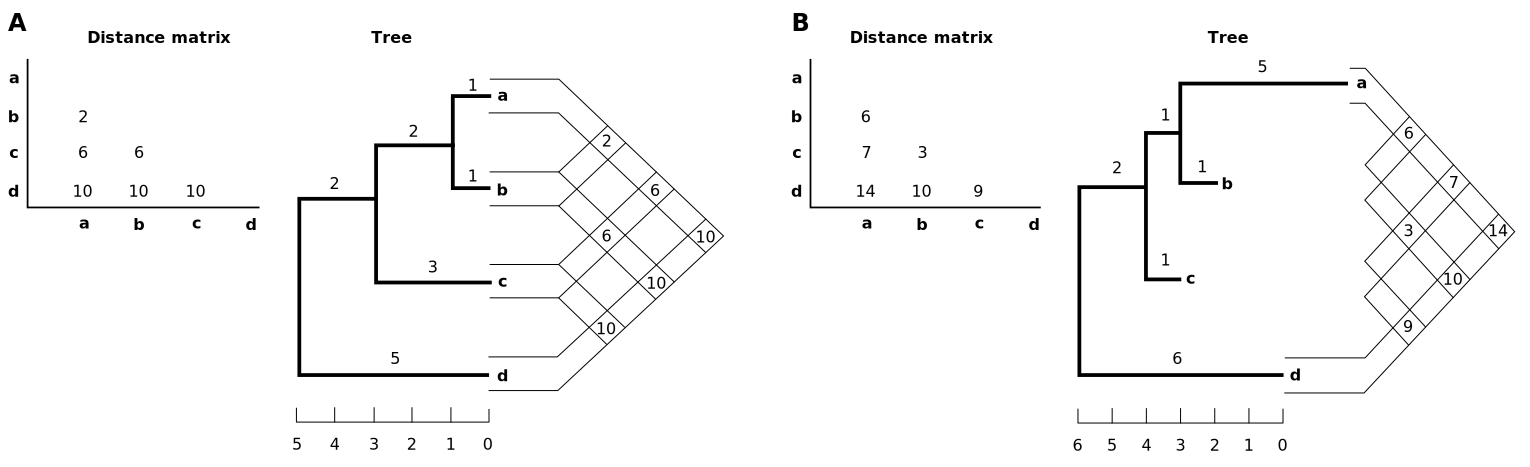
\includegraphics[width=1\linewidth]{files/ultrametric-distance-ddbcc8660c6e5afb67921cbbca262ddb.pdf}
\caption[]{Ultrametric distance matrix between four sequences a-d and the corresponding ultrametric tree (A).
Additive distance matrix between four sequences a-d and the corresponding additive tree (B).
Values in the distance matrix correspond to the sum of the branch lengths along the path between the two sequences on the tree, therefore this data is metric.
Credits: \href{https://creativecommons.org/licenses/by-nc/4.0/}{CC BY-NC 4.0} \cite{own_3_2024}.}
\label{ultrametric_distance_alt}
\end{figure}

Once these pairwise distances have been calculated, the MSA is not further used and trees are built directly from the distances (Figure~\ref{character_distance_alt}).
Unlike for the character-based trees, in distance-based trees it is not possible to assess what character contributed where on the tree, as all individual characters have been combined into one overall pairwise distance value.
Moreover, invariant characters (MSA positions containing no variation) \textit{do contribute} to the pairwise distance values.
This is a main difference with the character-based approach where only variant characters contribute to the tree.

Clustering methods have the advantage that they are fast and do not require vast computational resources (there is no tree space nor NP-completeness as for the character-based trees, outlined above (see Box 3[w3box3\_bifurcating])).
Clustering methods assign individuals to clusters in such a way that individuals in one cluster are more similar to each other than to those from other clusters.
There is no explicit score or optimality criterion, only the minimisation of overall distance across all sequences.
Clustering usually produces one tree, no alternative `equally good' trees are shown; this is due to the clustering algorithm which is designed to produce a single tree.

\begin{framed}
\textbf{Box 3.4: Distance measures and their qualities}\\
\begin{figure}[!htbp]
\centering
\includegraphics[width=0.375\linewidth]{files/distances-0a3e8103842dfb096f52aba307814e2a.png}
\caption[]{Credits: \href{https://creativecommons.org/licenses/by-nc/4.0/}{CC BY-NC 4.0} \newline
\cite{own_3_2024}}
\label{distances}
\end{figure}

\begin{figure}[!htbp]
\centering
\includegraphics[width=0.375\linewidth]{files/inequality_alt-084cf637e6e35dcf5c4f16a814a1c66d.pdf}
\caption[]{Credits: \href{https://creativecommons.org/licenses/by-nc/4.0/}{CC BY-NC 4.0} \newline
\cite{own_3_2024}}
\label{inequality_alt}
\end{figure}

Euclidean or metric distance (Figure~\ref{distances}) requires observed distances to be \textit{non-negative}, \textit{symmetrical}, \textit{distinct} and to obey the \textit{triangle inequality} (Figure~\ref{inequality_alt}, (left): the distance between any pair of sequences a and b cannot exceed the sum of the distances between those sequences and a third sequence c.

Ultrametric distances are characterised by \textit{ultrametric inequality} (Figure~\ref{inequality_alt}, right): the two largest distances, when comparing three sequences, are equal (in this case 6 = 6).
Ultrametric distances have the attractive characteristic that they evolve clock-like, and hence that the most similar sequences will also be most closely related.
In fact, the ultrametric tree (Figure~\ref{ultrametric_distance_alt}) perfectly describes the observed distances as shown in the distance matrix.
\end{framed}


\bigskip
\centerline{\rule{13cm}{0.4pt}}
\bigskip

\subparagraph{Neighbor Joining}\label{chapter3_neighbor_joining}

Probably the most commonly used distance tree building method is Neighbor Joining (NJ), which is fast and effective, especially for large MSAs (with hundreds of sequences).
NJ tree building starts with a fully unresolved tree, containing all sequences in an MSA, and calculates a total tree length (or overall starting distance) by summing all pairwise distances.
Subsequently, a pair of sequences is chosen and combined to start a small cluster (`neighbors') and the total tree length is updated, now replacing the two original by the joined taxa.
This step is repeated until all sequences and pairs are joined, whilst minimizing the overall distance (tree length) between them (Figure~\ref{neighbor-joining-process_alt}).

Neighbor Joining produces unrooted trees and therefore, if needed, outgroup rooting should be applied in order to root the tree.
There is no molecular clock assumption, which allows differences in branch lengths between neighbors (sisters) to be reconstructed.
NJ is implemented in \href{https://www.megasoftware.net/}{MEGA11}\cite{mega_2021}) and used in the practical.

% :::{figure} images/chapter3/neighbor-joining-kimura.png
%  :alt: Stepwise process involved in the neighbor joining computational process.
%  :width: 100%
%  :name: neighbor-joining-kimura
% 
%  Neighbor Joining.
%  An illustration of the computational process.
%  Tree length S is the sum of all branch lengths, and is minimized (F) by iteratively joining neighbors, starting from the star tree (A) (From Kimura 2004)
%  :::
% #% Unable to use figure neighbor-joining-kimura due to copyright

\begin{figure}[!htbp]
\centering
\includegraphics[width=1\linewidth]{files/neighbor-joining-pro-ce25f049379b59ccb378d7b30343ee7d.pdf}
\caption[]{Neighbor Joining.
An illustration of the computational process.
Tree length S is the sum of all branch lengths, and is minimized (F) by iteratively joining neighbors, starting from the star tree (A).
Credits: \href{https://creativecommons.org/licenses/by-nc/4.0/}{CC BY-NC 4.0} \cite{own_3_2024}.}
\label{neighbor-joining-process_alt}
\end{figure}

NJ is highly popular as it can generate trees with hundreds of terminals in a very short time.
This makes it a great tool for quickly assessing the (phylogenetic) structure in a data set (MSA) without having to explore wide tree spaces (as in the character-based approach).
It is good to keep in mind that NJ is a clustering method, i.e., it groups sequences on the basis of overall similarity, not on shared ancestry or synapomorphy.
Therefore, for phylogenetic studies, character-based analysis is preferred, and NJ analysis can be used in addition (Figure~\ref{neighbor_joining-aa}), to check for possible incongruencies between the two.
If these are found, it could mean that the data (the synapomorphies accumulated in the MSA) are not metric for that part of the tree, which could warrant additional analysis methods (such as phylogenetic network reconstruction) which is beyond the scope of this course.

\begin{figure}[!htbp]
\centering
\includegraphics[width=1\linewidth]{files/neighbor-joining-aa-72d1235eea811d9d1a82e7f19f33d304.jpg}
\caption[]{Neighbor Joining.
An unrooted NJ tree based on Myosin amino acid sequences.
The scale bar indicates 5\% sequence divergence.
Credits: \href{https://creativecommons.org/licenses/by/1.0/}{CC BY 1.0} \cite{neighbor_joining_aa_2000}.}
\label{neighbor_joining-aa}
\end{figure}


\bigskip
\centerline{\rule{13cm}{0.4pt}}
\bigskip

\subsubsection{Estimating sequence divergence}\label{chapter3_estimating_sequence_divergence}

In a phylogeny, when there is a combination of long terminal branches combined with short internal ones phylogenetic reconstruction is usually problematic when using nucleotides and parsimony analysis.
The reason for this is that on long branches (i.e., with highly-divergent sequences) the chance of any of the 4 nucleotides occurring in both branches at random, is actually quite high and can result in \textit{false synapomorphies}.
After some of these have accumulated, wrong clades can be the result.
This so-called \textit{long branch attraction} (LBA) artefact is fairly common, whenever isolated old lineages (such as \textit{Amborella} or \textit{Nymphaea} in the angiosperms) are involved but can also occur in gene trees.
LBA has been shown to be mitigated to some extent by \textit{modelling branch lengths}, rather than merely counting differences as branch length, as in parsimony where each substitution occurring in the MSA results in one extra step of treelength.
For the accurate estimation of branch lengths in a phylogenetic tree however we need accurate \textit{sequence divergence estimation}.

Evolutionary divergence (or distance) between homologous sequences is reflected in substitutions between them since splitting-off from their MRCA.
Intuitively, when comparing two sequences, one would just take the proportion of differing sites as sequence divergence, for instance, for a sequence of 1000 positions, having 10 differences would yield 0.01 or 1\% difference.
However, this so-called \textit{p-difference} does not necessarily consider \textit{all} substitutions that historically occurred during divergence of the two sequences (which may include reversals to the original state).
Estimating `true' sequence divergence means that we need to find substitutions that \textit{did} happen but are not visible in your MSA.
Variable sites can actually keep on changing during evolution, causing multiple substitutions to occur at the same position, which can lead to saturation of change.
In this way several substitutions may go unnoticed, and a mere \textit{p}-difference will underestimate actual sequence divergence.


\bigskip
\centerline{\rule{13cm}{0.4pt}}
\bigskip

\paragraph{Substitution models}

Substitution models, all based on the Jukes-Cantor (JC) formula given below, correct divergence estimates for unobserved events.
The JC formula is based on calculation of the chance of having a substitution for a particular site plus the chance of it not changing into any of the three other nucleotides for that site.
In the formula, $p$ stands for the observed proportion of differences (i.e., the \textit{p}-difference), and $d$ for the corrected divergence measure.
When all sites differ (i.e., $p = 1$), $d$ reaches 0.75 in the limit, i.e., the corrected $d$ cannot exceed 75\%.

\begin{equation}
d = -\frac{3}{4} \log{\left(1 - \frac{4}{3}p\right)}
\end{equation}

Figure~\ref{JC_alt} shows how the JC formula is applied in a \textit{model of substitution}, the JC model.
There is a matrix defining the six possible substitution types among the 4 nucleotide bases, i.e., T\leftrightarrowC, A\leftrightarrowG, A\leftrightarrowT, T\leftrightarrowG, C\leftrightarrowG, and C\leftrightarrowA.
In this case the relative rates for all six substitution types are assumed to be equal and denoted by one shared parameter, named `a'.
Another assumption in this model is that the base composition across the MSA is equal, assuming a 25\% probability of finding of each base at each position in each sequence.
The JC model is considered a fairly simple, one parameter, model.

% :::{figure} images/chapter3/JC.png
% :alt:
% :align: center
% :name: JC
% The Jukes Cantor model (left), transitions (blue) and transversions (red) and how they accumulate differently during evolutionary time (right) (From Zvelebil & Baum 2008).
% :::
% #% Unable to use figure JC due to copyright

\begin{figure}[!htbp]
\centering
\includegraphics[width=0.7\linewidth]{files/JC_alt-3246e60df7eeddaa4094ea98776fc4f0.pdf}
\caption[]{The Jukes Cantor model (left), transitions (blue) and transversions (red) and how they accumulate differently during evolutionary time (right).
Credits: \href{https://creativecommons.org/licenses/by-nc/4.0/}{CC BY-NC 4.0} \cite{own_3_2024}.}
\label{JC_alt}
\end{figure}

The first two substitution types listed above are \textit{transitions} (substitutions among the pyrimidines T and C, and among the purines A and G), whereas the other four occur between purines and pyrimidines and are referred to as \textit{transversions}.
The rate of transitions (\textit{ti}) has a different dynamic, and hence build-up of substitutions, compared with the rate of transversions (\textit{tv}) (see Figure~\ref{JC_alt}).
In the Kimura 2-parameter (K2P) model (Figure~\ref{K2P}) this is accounted for by adding an extra parameter  \textit{b}.
Parameter \textit{a} now estimates \textit{ti} ($P$) and parameter $b$ estimates \textit{tv} ($Q$); in the Kimura 2 Parameter formula, $P$ and $Q$ are the proportions of \textit{ti} and \textit{tv}, respectively:

\begin{equation}
d = \frac{1}{2} \ln{\left[ \frac{1}{1 - 2P - Q} \right]} + \frac{1}{4} \ln{\left[ \frac{1}{1 - 2Q} \right]}
\end{equation}

\begin{figure}[!htbp]
\centering
\includegraphics[width=0.375\linewidth]{files/K2P-c696dd10a2e3e6b29cdcb3abb91f60d1.pdf}
\caption[]{The Kimura 2-parameter substitution \newline
model with transitions indicated in \newline
orange (parameter \textit{a}) and transversions \newline
in blue (parameter \textit{b}). \newline
Note that base frequencies f\textsubscript{N} \newline
are considered equal in this model. \newline
Credits: \href{https://creativecommons.org/licenses/by-nc/4.0/}{CC BY-NC 4.0} \cite{own_3_2024}.}
\label{K2P}
\end{figure}

Besides the JC and K2P models, other models exist that take into account different aspects of DNA sequence evolution, such as differences between all six substitution types (\textit{general time reversible} or GTR), sequence base composition or nucleotide frequencies (\textit{Felsenstein81} or F81), and the distribution of rates of change in sites throughout the MSA: how many fast, and how many slow-evolving sites are there and how are they distributed (this is achieved by comparison with a gamma $\Gamma$ distribution).
The most complex models, with many parameters, will consist of combinations of all these aspects of DNA sequence evolution.
There are up to 220 different models to choose from.
It is good to realise that these models are reversible and therefore allow the reconstruction of unrooted trees only.
Once these are determined they can be rooted using outgroup rooting.

For amino acid sequence comparisons, instead of estimating parameter values from the data, amino acid substitution models are based on (pre-defined) \textit{substitution cost matrices} (see chapter~2) that are based on observations of amino acid substitutions found in over 30,000 protein sequences (e.g., the JTT, Blosum, Dayhoff, LG and WAG matrices).


\bigskip
\centerline{\rule{13cm}{0.4pt}}
\bigskip

\subsubsection{Maximum likelihood tree building}\label{chapter3_ML}

For character-based approaches these substitution models, as they are based on probabilities, allow us to calculate the \textit{likelihood} of our data supporting a particular tree and model.
This likelihood is a score describing how well data, tree and model fit together:

\begin{equation}
L = Pr(D|H)
\end{equation}

Or described in words: the likelihood $L$ is the probability of obtaining the data $D$ given hypothesis $H$, which includes the substitution model \textit{and} tree selected.
We could therefore also say:

\begin{equation}
L = Pr(\text{MSA} | \text{Tree, substitution model})
\end{equation}

Obviously, it is important to select the best fitting model for the data set (MSA).
Model selection proceeds by calculating the likelihood for your MSA using a range of different models and the same tree; the best resulting likelihood scores imply the best-fitting model.

Subsequently, a candidate tree is considered and the likelihood L\textsubscript{D} of observing the data (the MSA) is calculated given that model and that particular tree.
Then, another tree is considered whilst the same best-fitting model remains selected, and its parameter values are estimated again.
The likelihood L\textsubscript{D} of observing the data (your MSA) is calculated again and this time the likelihood may actually be better.
More trees are evaluated, and more model parameter values are considered, all the time keeping track of L\textsubscript{D} until no further increase L\textsubscript{D} can be obtained.
This is usually achieved by using the heuristic tree search approaches as outlined in Tree~space~and~heuristic~search~methods and depending on the tree space, determined by the number of sequences in the MSA.
The end result is the maximum likelihood estimate (MLE): the combination of a tree and model parameter values that maximizes the likelihood of the data.
This tree, which may not be the exact best MLE (it is after all heuristics), is then usually referred to as the ML tree.

Phylogenetic tree reconstruction based on MLE has become the dominant tree building approach over the past decade.
It is an efficient method that can consider differences in substitution rates and patterns between the sequences in an MSA.
This would mean that non-clocklike or biased (non-random) accumulation of substitutions would be modelled, and this would minimize possible artefacts in inferring the ML tree topology, for instance LBA (see above).

The MLE pipeline for phylogenetic reconstruction is implemented in the software package \href{http://www.iqtree.org/}{IQ-TREE} \cite{iqtree_2020}, which includes I) model testing, II) ML tree search, and III) bootstrapping for both nucleotide and amino acid sequences.
IQ-TREE will be demonstrated and used in this chapter's practical.

Finally, estimating evolutionary divergence using nucleotide substitution models can also be applied in a distance approach.
There, the substation models are applied to calculate `corrected' pairwise sequence distances, which are then used to produce a Neighbor Joining tree (see Figure~\ref{neighbor-joining-process_alt})


\bigskip
\centerline{\rule{13cm}{0.4pt}}
\bigskip

\paragraph{Model-testing, ML tree search, Bootstrapping}

After an ML tree with branch lengths has been obtained, there is still no information on how nodes in the ML tree may differ in terms of support by the data (MSA).
Therefore a bootstrap analysis is carried out, repeating the MLE process a number of times, based on pseudo-replicate data sets drawn from the MSA (see Nodal~support~in~phylogenetic~trees:~the~bootstrap).
After an ML tree is obtained for each pseudo-replicate data set, a 50\% majority-rule consensus tree is calculated in order to see the group frequencies (the proportion of replicates in which each node is occurring).
These frequencies are also referred to as \textit{bootstrap values}.
The idea is that the more synapomorphies a node has, the higher its bootstrap value will be.

Unfortunately, there is no simple linear relationship between character support and bootstrap values.
Generally, bootstrap values \textless  90\% are considered poor support for that node, and values \textless  50\% (or even \textless  60\%) as `no support'.
Bootstrap values of 62\% are usually obtained for MSAs containing one synapomorphy, meaning that such nodes should probably be ignored but this depends on the experience and interpretation of the analyst.
Figure~\ref{bootstrap_collapse_alt} illustrates what happens to bootstrap consensus trees when poorly supported nodes are collapsed: the tree topology becomes less well resolved but what is left is strong.
That is indeed the trade-off: visualizing lots of nice but poorly supported resolution \textit{versus} only focusing on strong nodes.
Usually, we want to see both.

% :::{figure} images/chapter3/bootstrap-collapse.jpg
% :alt: ML tree with bootstrap values and the same ML tree with low support bootstrap values collapsed.
% :width: 100%
% :name: bootstrap_collapse
% 
% Bootstrap analysis.
% A) A maximum likelihood tree with bootstrap values indicated at nodes.
% Note that not all nodes show a bootstrap value, which is probably because values <50% are ignored.
% B) The same analysis, but this time all nodes with bootstrap values <50% collapsed.
% Note the introduction of a polytomy containing four lineages resulting from collapsing weak nodes, and the change from additive tree to cladogram style in the collapsed tree. Credits: {cite}`bioinformatics_2007`.
% :::
% #% Unable to use figure bootstrap_collapse due to copyright.

\begin{figure}[!htbp]
\centering
\includegraphics[width=1\linewidth]{files/bootstrap-collapse_a-08a11a593959a3561c9871e2affed760.pdf}
\caption[]{Bootstrap analysis.
A) A maximum likelihood tree with bootstrap values indicated at nodes.
Note that not all nodes show a bootstrap value, which is probably because values \textless  50\% are ignored.
B) The same analysis, but this time all nodes with bootstrap values \textless  50\% collapsed.
Note the introduction of a polytomy containing four lineages resulting from collapsing weak nodes, and the change from additive tree to cladogram style in the collapsed tree.
Credits: \href{https://creativecommons.org/licenses/by-nc/4.0/}{CC BY-NC 4.0} \cite{own_3_2024}.}
\label{bootstrap_collapse_alt}
\end{figure}


\bigskip
\centerline{\rule{13cm}{0.4pt}}
\bigskip

\subsubsection{Recap tree building methods}

To summarize, tree building methods can be classified according to the type of data used, characters (or `sites') \textit{versus} pairwise distance, in which case we also refer to this as \textit{clustering} analysis.
Using characters for tree building results in applying an \textit{optimality criterion} in order to select among several (sometimes enormous numbers of) candidate trees.
Clustering usually results in a single tree, the optimality criterion approach in several, in which case a consensus tree is calculated.

Another useful criterion to classify tree building methods is whether an explicit model of character evolution is applied, versus mere counting (parsimony) of changes. In this course we covered Maximum Likelihood and parsimony, and Neighbor Joining using corrected distances, i.e., applying the character model in pairwise sequence comparison.
Bayesian Inference, in which probabilities for nodes are calculated, and different models are evaluated simultaneously, is beyond the scope of this course.
(If you are interested, they are covered in \href{https://wur.osiris-student.nl/onderwijscatalogus/extern/cursus}{BIS-40306 Comparative Biology \& Systematics}).

\begin{table}
\centering
\begin{tabular}{p{\dimexpr 0.333\linewidth-2\tabcolsep}p{\dimexpr 0.333\linewidth-2\tabcolsep}p{\dimexpr 0.333\linewidth-2\tabcolsep}}
\toprule
Data \rightarrow & Distances (pairwise) & Sites (characters) \\
\hline
\textbf{Approach} ↴ &  &  \\
Explicit model of character evolution & Neighbor Joining \newline
Neighbor Network & Maximum Likelihood \\
No model of character evolution & \textit{p}-difference & Parsimony(`counting') \\
Criterion? & Clustering & Optimality criterion \\
\bottomrule
\end{tabular}
\end{table}


\bigskip
\centerline{\rule{13cm}{0.4pt}}
\bigskip

\subsubsection{Practical assignments}

This guide contains questions and exercises to help you process the study materials of Chapter 3.
You have two mornings to work your way through the exercises.
In a single session you should aim to get about halfway through this guide, i.e., assignments I-IV.
Note that assignment VI is optional.

These practical exercises offer you the best preparation for the project in Week 6 and the tools and their use are also part of the exam material.
Thus, make sure that you develop your practical skills now, in order to apply them during the project and to demonstrate your observation and interpretation skills during the exam.

\textbf{Note, the answers will be published after the practical!}

\begin{framed}
\textbf{\textbf{Project Preparation Exercise}}\\
Using last chapter's ARF multiple sequence alignment (amino acid sequence),
aligned in MAFFT, now use MEGA 11 in order to make a NJ tree, using the
Poisson and then the Dayhoff model of amino acid substitutions.

Use FigTree to make a proper tree picture; then generate a Maximum likelihood
tree (with bootstraps) in IQ-TREE, and produce its pretty picture in FigTree.

Is the tree properly rooted? What outgroup could be added in case it is not
present yet?

Describe the following items in a few bullet points each.
You may include up to two figures or tables.

\begin{enumerate}
\item \textbf{Materials \& Methods} What did you do? Which data, databases and tools did you use, and why did you choose them? What important settings did you select?
\item \textbf{Results} What did you find, what are the main results? Report the relevant data, numbers, tables/figures, and clearly describe your observations.
\item \textbf{Discussion \& Conclusion} Do the results make sense? Are they according to your expectation or do you see something surprising? What do the results mean, how can you interpret them? Do different tools agree or not? What can you conclude? Make sure to describe the expectations and assumptions underlying your interpretation.
\end{enumerate}
\end{framed}

\subsubsection{Glossary}

This glossary contains the most important terms from this chapter.

\subsubsection{References}